\documentclass[border=2pt]{standalone}
\usepackage{tikz,amsmath}
\begin{document}
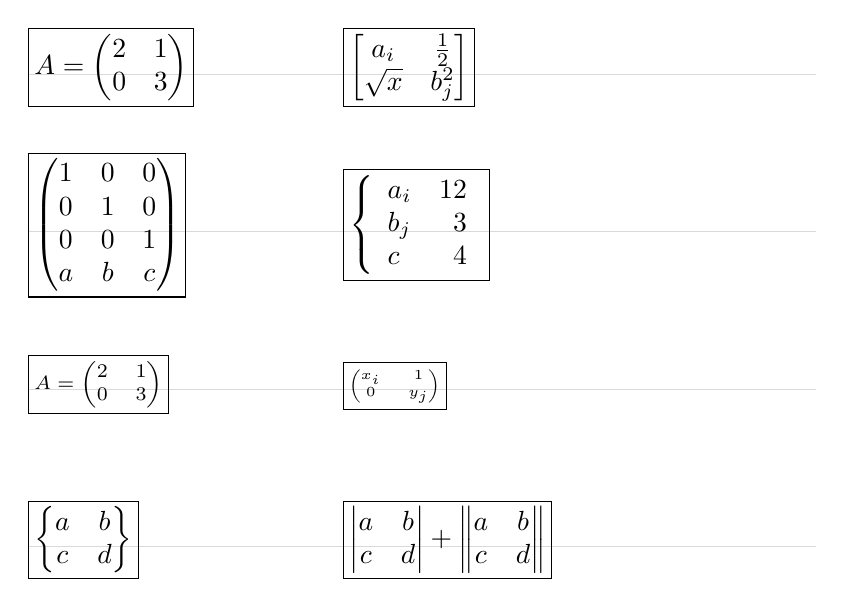
\begin{tikzpicture}
  \draw[gray!30] (0,0)--(10,0) (0,-2)--(10,-2) (0,-4)--(10,-4) (0,-6)--(10,-6);
  \node[anchor=base west,draw,inner sep=2pt] at (0,0) {$A=\begin{pmatrix}2&1\\0&3\end{pmatrix}$};
  \node[anchor=base west,draw,inner sep=2pt] at (4,0) {$\begin{bmatrix}a_i&\frac{1}{2}\\\sqrt{x}&b_j^2\end{bmatrix}$};
  \node[anchor=base west,draw,inner sep=2pt] at (0,-2) {$\begin{pmatrix}1&0&0\\0&1&0\\0&0&1\\a&b&c\end{pmatrix}$};
  \node[anchor=base west,draw,inner sep=2pt] at (4,-2) {$\left\{\begin{array}{lr}a_i&12\\b_j&3\\c&4\end{array}\right.$};
  \node[anchor=base west,draw,inner sep=2pt,font=\scriptsize] at (0,-4) {$A=\begin{pmatrix}2&1\\0&3\end{pmatrix}$};
  \node[anchor=base west,draw,inner sep=2pt,font=\tiny] at (4,-4) {$\begin{pmatrix}x_i&1\\0&y_j\end{pmatrix}$};
  \node[anchor=base west,draw,inner sep=2pt] at (0,-6) {$\begin{Bmatrix}a&b\\c&d\end{Bmatrix}$};
  \node[anchor=base west,draw,inner sep=2pt] at (4,-6) {$\begin{vmatrix}a&b\\c&d\end{vmatrix}+\begin{Vmatrix}a&b\\c&d\end{Vmatrix}$};
\end{tikzpicture}
\end{document}
